\documentclass[aps,prb,twocolumn,
	           groupedaddress,superscriptaddress,
               amsfonts,amssymb,amsmath,floatfix,
	           citeautoscript]{revtex4-1}


% --- PACKAGES ---
\usepackage{graphicx}
\usepackage[centering,hmargin=20mm,tmargin=28mm,bmargin=25mm]{geometry}
\usepackage{multirow}
\usepackage{newtxtext}
\usepackage[cmintegrals]{newtxmath}

%-----SI UNITS-----
\usepackage{siunitx}
\sisetup{range-phrase =\text{\,--\,},
	list-units   =single,
	range-units  =single,
	list-pair-separator = {\ \text{and}\ },
	list-separator = {,\ \linebreak[0]},
	list-final-separator = {,\ \linebreak[0]\text{and}\ }}

%--- REFERENCING ---
\usepackage{xcolor}
\usepackage{hyperref}
\hypersetup{colorlinks,
	linkcolor={blue!75!black!80!yellow},
	citecolor={blue!75!black!80!yellow},
	urlcolor={blue!75!black!80!yellow}
}

%--- CAPTIONS (sans serif) ---
\makeatletter
\renewcommand\@make@capt@title[2]{%
	\@ifx@empty\float@link{\@firstofone}{\expandafter\href\expandafter{\float@link}}%
	\sffamily{\textbf{#1}}\@caption@fignum@sep#2
}%
\renewcommand\figurename{Figure}
\makeatother

% --- SPACING ---
\usepackage{microtype} % Kerning and symbol-stretching
\usepackage{xspace}

\thickmuskip=5mu plus 2mu minus 1mu  %binary relations (default, 5mu plus 5mu)
\medmuskip=4mu plus 2mu minus 2mu    %binary operations (default, 4mu plus 2mu minus 4mu)

\frenchspacing %Ensure that revTeX does not do "double spaces" after punctuation

% --- COMMANDS ---
\renewcommand{\Im}{\operatorname{Im}}
\renewcommand{\Re}{\operatorname{Re}}
\newcommand{\sgn}{\operatorname{sgn}}

\newcommand{\iu}{\mathrm{i}}
\newcommand{\e}{\mathrm{e}}
\newcommand{\dd}{\mathrm{d}}
\newcommand{\unitvec}[1]{\ensuremath{\hat{\mathbf{#1}}}}
\newcommand{\sub}[1]{\ensuremath{_{\textrm{#1}}}} %Upright multi-character subscript
\newcommand{\super}[1]{\ensuremath{^{\textrm{#1}}}} %Upright multi-character superscript

%abbreviations
\newcommand{\ie}{i.e.\@\xspace} %Gobble-spaces of the "small" type (small is ensured by adding \@)
\newcommand{\cf}{cf.\@\xspace}
\newcommand{\eg}{e.g.\@\xspace}
\newcommand{\etc}{etc.\@\xspace}

\newcommand{\HarvardSEAS}{John A. Paulson School of Engineering and Applied Sciences, Harvard University, Cambridge, MA, USA}
\newcommand{\MITPhy}{Department of Physics, Massachusetts Institute of Technology, Cambridge, MA, USA}

% ----- COMMENTS AND META-ANNOTATIONS -----
\usepackage{textcomp} % for \textrightarrow
\usepackage{xifthen}
\usepackage{etoolbox}
\newboolean{togglecomments}
\newboolean{togglechanges} 

% toggle to true to see comments (otherwise hidden)
\setboolean{togglecomments}{true}  
% toggle to false to see mixed versions (otherwise edits are shown exclusively)
\setboolean{togglechanges}{false} 

\newcommand{\comment}[2]{%
    \ifbool{togglecomments}%
    {\textcolor{blue!70!black}{\small\textsf{%
    \textsuperscript{\textsc{\textsf{\MakeLowercase{#1}}}}%
    [#2]}}} % if true, show comments
    {}}     % if false, do nothing
\newcommand{\swap}[2]{\ifbool{togglechanges}
    {#2}  % TC-only version
    {\textcolor{red!70!black}{[#1]}\text{\textrightarrow{}}\textcolor{green!50!black}{[#2]}}}
\newcommand{\remove}[1]{\ifbool{togglechanges}
    {}    % TC-only version
    {\textcolor{red!70!black}{#1}}}
\newcommand{\inset}[1]{\ifbool{togglechanges}
    {{}#1}  % TC-only version
    {\textcolor{green!50!black}{{}#1}}}
\makeatletter
\newcommand{\citeremind}[1]{%
	\unskip%
    \textcolor{blue!75!black!80!yellow}{${}^\blacksquare$%
	\ifthenelse{\isempty{#1}}{}{\textsuperscript{\tiny\textsf{#1}}}%
	}\xspace}
\makeatother
\newcommand{\FIXME}[1]{\textcolor{red!70!black}{[#1]}}
\newcommand{\optional}[1]{\textcolor{yellow!70!gray}{#1}}





% --- DOCUMENT ---
\begin{document}

% --- TITLE & AUTHORSHIP ---
\title{Phonon polaritonics in two-dimensional materials}

\author{Nicholas Rivera}
\email{nrivera@seas.harvard.edu}
\affiliation{\HarvardSEAS}\affiliation{\MITPhy}
%
\author{Thomas Christensen}
\affiliation{\HarvardSEAS}\affiliation{\MITPhy}
%
\author{Prineha Narang}
\email{prineha@seas.harvard.edu}
\affiliation{\HarvardSEAS}

\date{\today}

% --- ABSTRACT ---
\begin{abstract}
    Extreme confinement of electromagnetic energy by phonon-polaritons holds the promise of strong and new forms of control over the dynamics of matter. 
    To bring such control to the atomic-scale limit, it is important to consider phonon-polaritons in two dimensional systems.  Recent studies have pointed out that in two-dimensional systems, splitting between longitudinal and transverse optical (LO and TO) phonons is absent at the $\Gamma$ point.  Does this lack of LO--TO splitting imply the absence of a phonon-polariton in polar monolayers? 
    Here, we derive a first-principles expression for the spatially non-local conductivity of a polar monolayer specified by the wavevector-dependent LO and TO phonon dispersions. In the long-wavelength (local) limit, we find a universal form for the conductivity in terms of the TO phonon frequency at the $\Gamma$ point, its lifetime, and the group velocity of the LO phonon. Our analysis reveals that the phonon-polariton of the bulk is essentially replaced by the LO phonon of the two-dimensional system. We calculate the confinement and propagation losses of the LO phonons, finding that high confinement and reasonable propagation quality factors coincide in regions which are difficult to detect with current near-field optical microscopy techniques. 
    Finally, we study the interaction of external emitters with two-dimensional hBN nanostructures, finding extreme enhancement of spontaneous emission due to coupling with localized 2D LO phonons, and the possibility of multi-mode strong and ultra-strong coupling between an external emitter and hBN phonons. Using the strong electromagnetic interactions between emitters and 2D LO phonons calculated in this work, it is now possible to design new hybrid states of light, electrons and phonons based on quantum electrodynamical strong coupling. 
\end{abstract}

\maketitle

% --- INTRODUCTION ---
Phonon-polaritons, hybrid quasiparticles of photons and optical phonons supported in polar materials, hold tremendous promise for deeply sub-diffraction control of electromagnetic fields at mid-infrared and terahertz frequencies. Qualitatively, phonon-polaritons share many features with plasmon-polaritons in conductors. Recently, it has been shown that phonon-polaritons enable confinement of light to volumes over $10^6$ times smaller than that of a diffraction-limited photon in free-space\cite{caldwell2013low,xu2014mid,caldwell2014sub,dai2014tunable,tomadin2015accessing,yoxall2015direct,li2015hyperbolic,dai2015subdiffractional,dai2015graphene,caldwell2015low,li2016reversible,Basov:2016,basov2017towards,low2017polaritons,giles2017ultra,li2018infrared,ma2018plane}. Due to this remarkable confinement and their relatively high lifetimes of around picoseconds, phonon-polaritons open new opportunities for vibrational spectroscopy,\cite{autore2018boron} radiative heat transfer~\cite{hillenbrand2002phonon}, and control of dynamics in quantum emitters~\cite{kumar2015tunable,rivera2017making,kurman2018control}. 
In many cases, extreme confinement of phonon-polaritons is achieved by the use of thin-films, which shrink the in- and out-of-plane wavelength of polaritons monotonically with decreasing film thickness~\cite{dai2014tunable,dubrovkin2018ultra}. A monolayer is the ultimate, atomic-scale limit of this effect when the properties of the bulk material can be used in the monolayer limit. In polar materials, the transition from 3D to 2D is not so simple, as in a polar monolayer, the LO--TO splitting that gives rise to phonon-polaritons in three-dimensions is absent at the $\Gamma$ point~\cite{sanchez2002vibrational,mele2002electric,serrano2007vibrational,sohier2017breakdown}. This raises a fundamental question about whether strongly confined electromagnetic modes exist in polar monolayers at all. 

In this Letter, we develop a theoretical and computational framework with quantitative, concrete examples to enable a new understanding of optical phononics in two-dimensional materials. We do so by deriving a universal form for the conductivity of a polar monolayer,  which depends solely on the LO and TO phonon frequencies---and their dispersion with momentum---in the two-dimensional system. Using parameters from Ref.~\citenum{sohier2017breakdown} for the canonical two-dimensional polar monolayer --- hexagonal boron nitride (hBN) --- we present the confinement and propagation losses of the 2D phononic modes, identifying the frequency region where they should be most easily detected. Finally, we show that these modes enable extreme light-matter interaction between emitters and polar materials, showing that for atom-like emitters, their spontaneous decay can be enhanced by up to eight orders of magnitude by the emitter--LO phonon coupling. For an infrared emitter with a sufficiently high free-space radiative decay rate ($> 10^6 s$ $^{-1}$), the enhanced linewidth of the emitter becomes comparable to the spacing between different phonon polaritonic resonances of an hBN nanostructure. This suggests the possibility of realizing the multi-mode strong coupling and ultra-strong coupling regimes of quantum electrodynamics in a two-dimensional hBN platform. Our results for hBN are particularly relevant due its widespread use in 2D van der Waals heterostructures. In addition to providing functionality as a layer which improves the electrical and optical properties of other 2D materials, such as graphene, our results suggest that in these heterostructures, the hBN layers could provide a platform for nanophotonics and quantum optics which operates in the mid-infrared spectral range. 

\section{Optical response of optical phonons in two-dimensions}
In this section, we develop a theory of electromagnetic response due to optical phonons in two-dimensional systems. The key prediction is the conductivity of the monolayer. To obtain it, we consider the response of the ions of the monolayer due to a longitudinal electromagnetic potential $\phi$. The interaction Hamiltonian in this case is
\begin{equation}
    H_{\mathrm{int}} = \int \dd^2x ~\rho \phi = -\int \dd^2x~ (\nabla\cdot\mathbf{P})\phi,
    \label{eq:coupling}
\end{equation} 
with $\rho$ the induced charge density and $\mathbf{P}$ the total polarization density associated with the ionic motion. 
Within linear response theory, the induced polarization density can be straightforwardly evaluated from the displacement amplitude $\mathbf{u}_{\kappa}$ of every atom $\kappa$ within the unit cell. Specifically, to first order, the induced polarization is (in repeated-index notation):
\begin{equation}
    P_i - P_i^{0} = \frac{\partial P_i}{\partial u_{\kappa,j}}u_{\kappa,j} \equiv \frac{1}{\Omega}Z_{\kappa,ij}u_{\kappa,j},
\end{equation} 
where $Z_{\kappa,ij} \equiv \Omega\frac{\partial P_i}{\partial u_{\kappa,j}} $ is the Born effective charge tensor of ion $\kappa$ and $\Omega$ is the unit cell area. $P_i^{0}$ is the equilibrium polarization in the absence of displacements, which is zero here. With this relation between polarization and ionic displacements, the interaction Hamiltonian in Equation~\eqref{eq:coupling} couples the scalar potential and the ionic displacements.  We consider the response of the monolayer to a scalar potential of the form $\phi(\mathbf{r}) = \phi(\mathbf{q},\omega)\e^{\iu\mathbf{q}\cdot\mathbf{r}-\iu\omega t}$, where $\mathbf{q}$ is a two-dimensional wavevector in the plane of the monolayer. Such a potential corresponds to a longitudinal electric field  $\mathbf{E}(\mathbf{r}) = \iu\mathbf{q}\phi(\mathbf{r})$. 

In what follows, we assume the validity of the random-phase approximation (RPA) in calculating Coulombic interactions between ions in the polar lattice. Within the RPA, these Coulombic interactions are accounted for by taking the induced polarization $\mathbf{P}(\mathbf{q},\omega)$ to be proportional \emph{total} electric field, $\mathbf{E}_{\mathrm{tot}}(\mathbf{q},\omega)$, defined to be the sum of the externally applied electric field and the electric field created by the induced polarization. The polarization and total-field are connected by the polarization-polarization response (tensor) function  $\boldsymbol{\Pi}(\mathbf{q},\omega)$ via
\begin{equation}
\mathbf{P}(\mathbf{q},\omega)  = \epsilon_0\boldsymbol{\Pi}(\mathbf{q},\omega)\mathbf{E}_{\mathrm{tot}}(\mathbf{q},\omega),
\end{equation}
where boldfaced quantities refer to vectors or tensors as appropriate. The polarization-polarization response function is related to the conductivity via the relation $\boldsymbol{\sigma}(\mathbf{q},\omega) = -\iu\omega\epsilon_0\boldsymbol{\Pi}(\mathbf{q},\omega)$. From the Kubo formula, it follows that the conductivity is
\begin{equation}\label{eq:2dsusceptibility}
    \boldsymbol{\sigma}(\mathbf{q},\omega) =  \frac{-\iu \omega}{ \Omega\mathcal{Z}}\sum\limits_{m,n}\frac{\mathbf{P}_{mn}(\mathbf{q})\otimes\mathbf{P}_{nm}(\mathbf{q})}{\hbar\omega + E_{nm}+\iu 0^+}\Big(\e^{-\beta E_m}-\e^{-\beta E_n} \Big),
\end{equation}
where $m,n$ are states of the phononic Fock space of the monolayer, $P_{mn,i}(\mathbf{q}) = \sum_{\kappa,j}Z_{\kappa,ij}\langle m | u_{\kappa,j}(\mathbf{q}) | n \rangle$ are matrix elements of the polarization associated with phonon modes (where $u_{\kappa,j}(\mathbf{q})$ is the Fourier transform of the phonon displacement operator), $E_{m}$ ($E_n$) is the energy of state $m$ ($n$), $\beta \equiv 1/k_{\text{\textsc{B}}}T$ is the inverse temperature, and $\mathcal{Z}$ is the grand partition function. We now evaluate the contribution of optical phonons to the polarization-polarization response in the low-temperature limit $T << \frac{\hbar\omega_{\mathrm{ph}}}{k_B}$ with $\omega_{\mathrm{ph}}$ a characteristic optical phonon frequency.  Taking a material with long-wavelength isotropy, such as hBN, we only have to consider the $qq$-component in the response tensor, where $qq$ denotes a pair of directions parallel to the wavevector. Denoting $\sigma_{qq}$ as simply $\sigma$, we find that the conductivity is given by \cite{rivera2018ab}: 
\begin{equation}
    \sigma(\mathbf{q},\omega) = \frac{-\iu\omega}{\hbar\Omega} \frac{2\omega_{\mathbf{q},\mathrm{L}}}{\omega^2_{\mathbf{q},\mathrm{L}}-\omega^2-\iu\omega\tau^{-1}}|\hat{\mathbf{q}}\cdot\langle 1_{\mathbf{q},\mathrm{L}}|\mathbf{P}(\mathbf{q})|0_{\mathbf{q},L}\rangle|^2,
    \label{eq:polpolresponse}
\end{equation}
where L-subscripts denote longitudinal polarization, $|0_{\mathbf{q},\mathrm{L}}\rangle$ ($|1_{\mathbf{q},\mathrm{L}}\rangle$) denotes a state with no (one) longitudinal phonon of wavevector $\mathbf{q}$, and $\hat{\mathbf{q}}$ denotes a unit vector in the direction of $\mathbf{q}$. We have also phenomenologically included the phonon dissipation rate $\tau^{-1}$, consistently with  a relaxation-time prescription.  The frequency $\omega_{\mathbf{q},\mathrm{L}}$ in the denominator, as in the case of bulk phonons, is the frequency of the longitudinal phonon of wavevector $\mathbf{q}$ prior to considering LO--TO splitting \cite{BornHuang:1954}.
This is consistent with the fact that LO--TO splitting is a collective effect arising from Coulomb interactions and the fact that the equation above represents a single-particle susceptibility. Coulomb interactions are accounted for in the random phase approximation, and to include them in the single-particle response amounts to an uncontrolled double-counting. 

Next, we express the polarization matrix element in Equation~\eqref{eq:polpolresponse} in terms of the Born effective charges of the monolayer and the phonon displacement eigenvectors. Considering the longitudinal phonon contribution to the second-quantized ionic displacement, as in Ref.~\citenum{srivastava1990physics}, we find that the conductivity within the RPA is given by
\begin{equation}
    \sigma(\mathbf{q},\omega) = -\frac{\iu\omega }{\Omega}\frac{\Big|\hat{\mathbf{q}}\cdot\sum\limits_{\kappa}\mathbf{Z}_{\kappa}\boldsymbol{\eta}_{\kappa} \Big|^2}{\omega^2_{\mathbf{q},\mathrm{L}}-\omega^2-\iu\omega\tau^{-1}}
    \label{eq:conductivity_simplified}
\end{equation}
  In this expression, $\omega_\mathrm{L}$, the LO phonon frequency prior to LO-TO splitting, has been re-named as $\omega_{\mathrm{TO}}$, the transverse optical phonon frequency, because in the absence of LO--TO splitting, they are degenerate. This is done in order to make the form of the final results more closely resemble their 3D counterparts. 
Additionally, we have defined scaled eigendisplacements $\boldsymbol{\eta}_{\kappa\mathbf{q}}\equiv \frac{\hat{\mathbf{e}}_{\kappa\mathbf{q},\mathrm{L}}}{\sqrt{M_{\kappa}}}$, where $\hat{\mathbf{e}}_{\kappa\mathbf{q},\mathrm{L}}$ is the unit-normalized polarization vector of atom $\kappa$ in the unit cell oscillating according to a longitudinal phonon of wavevector $\mathbf{q}$ and $M_{\kappa}$ is the mass of atom $\kappa$. 

While the conductivity is the main electromagnetic quantity of interest for electrodynamics applications, we briefly state the form of the (2D) permittivity, as its zeros immediately yield the longitudinal modes of the system, which are the LO phonons. The permittivity within the RPA, denoted $\epsilon_{\textrm{RPA}}$ is related to the polarization-polarization response function via \cite{jablan2009plasmonics} $\epsilon_{\textrm{RPA}} = \epsilon_{\mathrm{env}} + \frac{1}{2}q\Pi(q,\omega)$ and the conductivity via $\epsilon_{\textrm{RPA}} = \epsilon_{\mathrm{env}} + \frac{\iu q\sigma(q,\omega)}{2\omega\epsilon_0}$. Here, $\epsilon_{\mathrm{env}}$ is the average permittivity of the bulk above and below the monolayer, and is added to take into account the polarization arising from these bulk materials. Based on Equation~\eqref{eq:conductivity_simplified}, the zeros $\omega_{\mathbf{q}}$ of the RPA dielectric function satisfy:
\begin{equation}
    \omega^2_{\mathbf{q}} - \omega^2_{\mathrm{TO}} = V(q)\frac{1}{\Omega}q^2\Big|\hat{\mathbf{q}}\cdot\sum\limits_{\kappa}\tilde{\mathbf{Z}}_{\kappa}\boldsymbol{\eta}_{\kappa}\Big|^2,
    \label{eq:zerosofresponse}
\end{equation}
  where $V(q)$ is the Coulomb interaction in Fourier space, which in two dimensions, is given by $V(q) = \frac{e^2}{2\epsilon_0\epsilon_{\mathrm{env}}q}$. Given that the zeros of the dielectric function are associated with longitudinal modes, one expects that $\omega_{\mathbf{q}}$ is in fact the frequency of the LO phonon mode. This is consistent with the result of Ref.~\citenum{sohier2017breakdown}, in which \relax{{}\ } \citeauthor{sohier2017breakdown} show that in two-dimensional polar materials, the extra restoring forces on LO phonons relative to TO phonons, due to the Coulomb interaction, lead to a wavevector-dependent LO--TO splitting and zero LO--TO splitting at the $\Gamma$ point of the Brillouin zone. 
  
Given these results, we now re-express the conductivity explicitly in terms of the 2D phonon dispersion, and derive a universal form for the conductivity in the local ($q\rightarrow 0$) limit specified in terms of three parameters: the TO phonon frequency, the group velocity of the LO phonon at the $\Gamma$ point, and the damping rate. From Equation (7), we can immediately write the conductivity as
  \begin{equation}
  \sigma(q,\omega) = \frac{-2\iu\epsilon_0\epsilon_{\mathrm{env}}}{q}\frac{\omega^2_{\mathbf{q},\mathrm{LO}}-\omega^2_{\mathrm{TO}}}{\omega^2_{\mathrm{TO}}-\omega^2-\iu\omega\tau^{-1}}.
  \end{equation}
 For small $q$,  the Born charges are (to lowest-order) constant, and so the LO phonon dispersion takes the form $\omega_{\mathbf{q},\mathrm{LO}}=\sqrt{\omega^2_{\mathrm{TO}}+2v_g\omega_{\mathrm{TO}}q} \approx \omega_{\mathrm{TO}} + v_gq$, where $v_g$, the LO phonon group velocity, is defined from microscopic parameters through the relation
 \begin{equation}
    v_{\mathrm{g}} = \frac{e^2 }{4\epsilon_0 \epsilon_{\mathrm{env}}\omega_{\Gamma, \mathrm{TO}}\Omega}\Big|\sum\limits_{\kappa,j}Z^r_{\kappa,ij}\eta_{\kappa,j}  \Big|^2. 
\end{equation}
Thus, in the long wavelength limit, we have the following universal parameterization of the conductivity of a polar monolayer:
\begin{equation}
    \sigma(\omega) =  \frac{-4\iu\epsilon_0\epsilon_{\mathrm{env}}\omega_{\mathrm{TO}}v_g}{\omega^2_{\mathrm{TO}}-\omega^2-\iu\omega\tau^{-1}}.
    \label{eq:localsigma}
\end{equation}
From this relation, it follows that given the properties of the 2D phonons (from experiments or from \emph{ab initio} calculations), one can immediately specify the conductivity. Alternatively, from optical measurements (including far-field measurements) which allow one to extract the conductivity, it becomes possible to extract the group velocity of 2D LO phonons and thus the small-wavevector dispersion of those phonons. 
  
Before moving on to analyze the electrodynamics of 2D phonon-polaritons, we make two comments on lack of LO--TO splitting in 2D polar materials. The first is that this situation is in stark contrast to the situation of polar materials in 3D, which have a finite LO--TO splitting at the $\Gamma$ point. In the absence of such LO--TO splitting in 3D, there would be no frequency compatible with the existence of a phonon  polariton. On the contrary, we will show that in 2D, despite the absence of LO--TO splitting at the $\Gamma$ point, there persists a strongly confined evanescent electromagnetic mode with a high local density of states which in all respects is similar to a phonon polariton of a thin film, but is in fact the 2D LO phonon of the polar monolayer.

The second comment is that much of what has been discussed here has a strong analogy with the theory of optical response in electron gases in 2D, and particularly the relation between plasmons in 2D and 3D. To elaborate on this analogy, To do so, we take Equation (7) in the case of a two-atom unit cell (such as hBN), and note that the term in the sum over Born charges can be written as $e^2\big|\sum_{\kappa,j}Z^r_{\kappa,ij}\eta_{\kappa,j}  \big|^2 \equiv  \Big(\frac{eZ^r_*}{\sqrt{M_*}}\Big)^2 \equiv \Big(\frac{Q_*}{\sqrt{M_*}}\Big)^2$. Then, the LO--TO splitting can be written as $\omega^2_{\mathbf{q}} - \omega^2_{\mathbf{q},\mathrm{TO}} = \frac{Q_*^2}{2\epsilon_0\epsilon_{\mathrm{env}} M_*}q$. Now we note that the RHS is exactly the squared-frequency $\omega^2_{\mathbf{q}p}$ for a plasma oscillation in a 2D gas of charged particles with charge $Q_*$ and mass $M_*$. This squared frequency can be thought of as the ``LP--TP'' splitting between longitudinal and transverse plasma oscillations. Of course, there are no transverse plasma oscillations due to the structure-less nature of the electron, and so ``$\omega_{\mathrm{TP}}"$  should be considered as 0. In the three-dimensional plasmon case, `$\omega_{\mathrm{TP}} = 0$', but the difference between the squared longitudinal and transverse plasma oscillation frequencies at zero-wavevector is non-zero and given by $\omega_p^2$. In other words, the plasma frequency in electron gases is analogous to the LO--TO splitting in polar materials. The change in the dispersion of 3D versus 2D plasmons, like 3D versus 2D LO phonons, arises from the change in dimensionality of the Coulomb interaction from 3D to 2D.  This analogy between phononic and plasmonic behavior as a function of dimension is illustrated schematically in Figures~\ref{fig:1}(b,c).
  
\section{Electrodynamics of optical phonons in two-dimensions}
To relate for example the polarization-polarization response function  to the electromagnetic modes supported by a polar monolayer, we solve Maxwell's equations for an evanescent electromagnetic mode supported by a surface with polarization-polarization response tensor $\mathbf{\Pi}$. We consider the monolayer to be sandwiched by a superstrate of permittivity $\epsilon_+$ and a substrate of permittivity $\epsilon_-$. To strip the analysis to its bare essentials, we consider optical phonon response with in-plane isotropy in the long-wavelength limit arising from in-plane LO oscillations. A relevant example of a system where these conditions are satisfied is in a hexagonal boron nitride monolayer (see Figure~\ref{fig:1}(a) for schematic atomic structure). In a monolayer geometry with translation invariance and in-plane isotropy, the solutions of Maxwell's equations can be decomposed into transverse magnetic (TM) and transverse electric (TE) parts, where the magnetic or electric field respectively is transverse to the in-plane wavevector of the mode. In practice, it is the TM mode which is associated with highly confined electromagnetic waves that are of use in nanophotonics.  Given the isotropy, we may suppress indices from the response tensor. We may also consider without loss of generality a TM mode with wavenumber $q$ along the $x$-direction in the monolayer and magnetic field $H(z)\e^{\iu qx-\iu\omega t}$ along the $y$-direction of the monolayer. The direction transverse to the monolayer is denoted as $z$.  With these definitions in place, the Maxwell equation satisfied by the magnetic field is 
\begin{equation}\label{eq:2dmaxwell}
    \bigg(-\frac{\dd^2}{\dd{}z^2}+q^2-\epsilon_{\pm}\frac{\omega^2}{c^2} \bigg)H(z) = 0,
\end{equation}
where $\epsilon_1$ applies for $z>0$ and $\epsilon_2$ applies for $z<0$.
%\comment{tc}{Probably makes sense to use $\varepsilon_+$ instead of $\varepsilon_1$ and $\varepsilon_-$ for $\varepsilon_2$, to have just a single class of subscripts for this notion.}
We consider a solution of the form $H(z) = h_\pm\e^{\mp\kappa_\pm z}$ with $\kappa_\pm = \sqrt{q^2-\epsilon_{\pm} k_0^2}$ with $\pm$ corresponding to $\pm z > 0$ respectively.  The boundary condition on the magnetic field is $h^+-h^- = -K_x = \iu\omega\mathbf{P}_x$ where $\mathbf{K}$ is the surface current density, expressed through the polarization density $\mathbf{P}$ of the monolayer.  This condition enforces $\frac{h^-}{h^+} =(1+\frac{\epsilon_0}{\epsilon_-} \kappa_-\Pi)^{-1}$. 
Continuity of the electric field in the $x$ direction enforces $\frac{\epsilon_-}{\epsilon_+} = -\frac{\kappa_-}{\kappa_+}\frac{h^-}{h^+}$. 
Combining the two conditions, we obtain the usual dispersion equation for the TM mode of a polarizable 2D monolayer, namely $\epsilon_+/\kappa_+ + \epsilon_-/\kappa_- +\epsilon_0\Pi=0$. Given the deeply subwavelength nature of 2D phonon-polaritons, \ie since $q\gg\omega/c$ such that $\kappa_{\pm}\simeq q$, the dispersion equation can be reduced to its quasistatic limit without consequential loss of accuracy:
\begin{equation}
    \epsilon_{\mathrm{env}} + \frac{1}{2}\epsilon_0 q \Pi(q,\omega) \equiv \epsilon_{\mathrm{RPA}}(\omega) = 0,
    \label{eq:dispeq}
\end{equation}
with $\epsilon_{\mathrm{env}}\equiv (\epsilon_++\epsilon_-)/2$. Thus, the condition for `phonon-polaritons' coincides precisely with the condition for longitudinal optical phonons.  Thus, one of the main results of our manuscript is that despite the lack of LO--TO splitting at the $\Gamma$ point, there nevertheless exists a strongly confined evanescent mode in many respects similar to the phonon-polaritons of thin films. We now analyze the dispersion relation of phonon polaritons in a specific material, hexagonal boron nitride, in more detail, showing the possibility of highly confined electromagnetic modes with a large local density of states. 

\begin{figure}[t]
    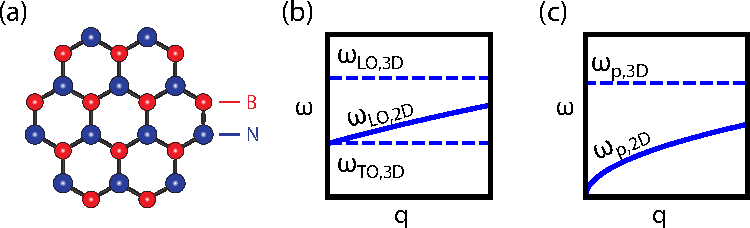
\includegraphics[width=85mm]{fig1.pdf}
    \caption{%
        \textbf{LO phonons as the basic electromagnetic waves of a polar monolayer.} (a) Schematic structure of a polar monolayer such as hexagonal boron nitride. (b) Properties of LO and TO phonons in 3D and 2D. In 3D, there is a finite LO--TO splitting at zero wavevector, while in 2D there is none. Despite this, the 2D LO phonon plays the role of the phonon-polariton in 3D and thin films. (c) Analogous physics appears in electron gases in 3D and 2D, where the 3D plasma frequency is similar to the 3D LO--TO splitting. In 2D, the plasma frequency at zero wavevector is zero, but the electromagnetic physics is determined by the dispersion of 2D plasmons, which replace the plasmon polariton of bulk and thin films.
        %\comment{tc}{We already discussed reasonable changes to the figures in-person, so I won't comment on that this time around.}
        \label{fig:1}
        }
\end{figure}~


\begin{figure*}[t]
    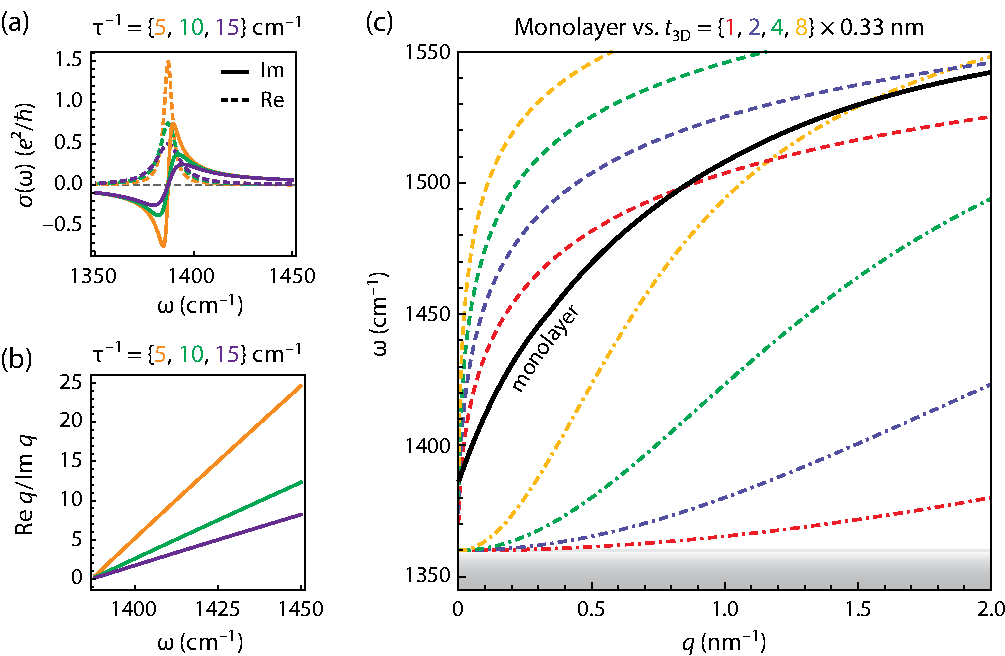
\includegraphics[width=135mm]{figure2hBN.pdf}
    \caption{%
        \textbf{Properties of phonon polaritons in an monolayer of boron nitride compared to bulk.} (a) Real and imaginary parts of the conductivity of 2D hexagonal boron nitride in units of $e^2/\hbar$ for different values of the loss-rate. (b) Propagation quality factor, which measures the number of wavelengths of propagation of the 2D phonon polariton. (c) Dispersion relation of phonon polaritons in the monolayer (black) and thin films whose thicknesses are taken to be 1,2,4, and 8 interlayer spacings in hBN. For the thin-film, the fundamental mode and the first higher-order mode are plotted. 
        \label{fig:2}
        }
\end{figure*}

\section{Properties of 2D LO phonon modes in monolayer hBN}

In Figure ~\ref{fig:2}(a), we present the conductivity of 2D hBN of Eq.~\ref{eq:localsigma}, using parameters from Ref. $\cite{sohier2017breakdown}$ calculated from density functional theory within the local density approximation. From the conductivity, the dispersion relation of phonon polaritons on an infinite sheet is given by $q=\frac{2\iu\omega\epsilon_0\epsilon_{\mathrm{env}}}{\sigma(\omega)}$. The dispersion, assuming $\tau = \infty$, and $\epsilon_{\mathrm{env}}=1$ is shown in \ref{fig:2}(c) (black line). A key figure of merit for applications involving the propagation of phonon polaritons, is the propagation quality factor, defined by $\frac{\text{Re }q}{\text{Im }q} = \frac{\text{Im }\sigma(\omega)}{\text{Re }\sigma(\omega)}$, which is shown in \ref{fig:2}(b).

For monolayer hBN, the wavevector grows very rapidly with frequency, due to the extremely low group velocity of 2D LO phonons, which is a remarkable four orders of magnitude slower than the speed of light. In particular, at frequencies of \SI{1450}{\per\cm}, the phonon-polariton has a wavelength of about 15 nm, which is much shorter wavelength than any phonon-polariton measured so far, and, similarly shorter than any plasmonic wavelength, even in graphene. In fact, this short a wavelength is essentially out of the range of measurability beyond the range of current scattering near-field microscope (SNOM) measurements, which are limited (by tip radii) to wavelengths greater than $\approx\,\SI{60}{\nm}$. The 2D LO phonon-polariton could in principle be measured by SNOM closer to the TO frequency, where confinement is smaller; unfortunately, as shown in Figure~\ref{fig:2}(b), near the TO frequency, dissipation is far higher (and corresponding propagative quality factors $\Re q/\Im q$ far lower) due to large $\Re\sigma$ (or, equivalently, large $\Im\epsilon_{\mathrm{RPA}}$).

These considerations imply that access to the lower-loss and higher-confined portions of the dispersion relation of phonon-polaritons, in the absence of a sharp tip, requires a near-field probe such as a free electron probe, as used in electron energy loss spectroscopy (EELS), where slow electrons can be used to probe plasmon wavelengths of just a few nanometers in monolayer metals, as well as the nonlocal bulk plasmon dispersion in metals~\cite{nagao2001dispersion,de2010optical,diaconescu2007low}.
EELS has been recently employed to measure phonon-polaritons in ultrathin films of hBN~\cite{govyadinov2017probing}. Another interesting class of near-field probes, with relevance to fundamental physics and quantum optics applications, is a quantum emitter such as an atom, molecule, or quantum well. Recently, it was demonstrated using nanostructures of bulk hBN that the interaction of vibrational emitters with phonon-polaritons is on the border of the strong coupling regime~\cite{autore2018boron}.

In the rest of this section, we discuss the relation between the dispersion of an hBN monolayer versus the atomically-thick limit of a thin film of a material with hBN's bulk dielectric function. To aid this discussion, in \ref{fig:2}(c), we show the dispersion relation of thin films of `bulk' hBN with film thicknesses of 1, 2, 4, and 8 times the interlayer spacing of bulk hBN, which is roughly 0.33 nm. For these plots, we take hBN to be cleaved such that the optic-axis is perpendicular to the plane of the film. In such a case, the components of the bulk permittivity perpendicular and parallel to the c-axis ($\epsilon_{\perp}$ and $\epsilon_{||}$ respectively) are given by
\begin{equation}
\epsilon_{\perp,||}(\omega) = \epsilon_{\infty\perp,||}\left(1 + \frac{\omega^2_{\mathrm{LO}\perp,||}-\omega^2_{\mathrm{TO}\perp,||}}{\omega^2-\omega^2_{\mathrm{TO}\perp,||}} \right),
\end{equation}
with $\epsilon_{\infty\perp,||} = 2.95, 4.87$, $\omega_{\mathrm{TO}\perp,||} = 760,1360$ cm$^{-1}$, and $\omega_{\mathrm{LO}\perp,||} = 830,1614$ cm$^{-1}$ \cite{caldwell2014sub,dai2014tunable}. Losses are ignored in this discussion altogether. In the range between $\omega_{\mathrm{TO}}$ and $\omega_{\mathrm{LO}}$, the corresponding component of the permittivity is negative, while the other component is positive. This hyperbolicity leads to a dispersion for hBN thin films that have multiple branches at a given frequency, as can be seen in \ref{fig:2}(c).  This trend persists even when the thickness of the bulk is taken down to a single layer, albeit being pushed to high wavevectors. This is in contrast with the true monolayer, in which there is only one LO phonon mode. Given that the phonon polariton of 2D is the LO phonon, there can be only one branch of the dispersion. Another anomaly between 2D and 3D is that the dispersion relation of the 2D LO phonon is non-monotonic, and the frequency starts to decrease for sufficiently large wavevector. This can never happen by extrapolating to a monolayer a dielectric function which has finite LO--TO splitting. This `turn-back' point corresponds to a frequency of around $1500$ cm$^{-1}$ and a phonon wavelength of less than 1 nm. Thus, this deviation is unlikely to be probed in typical optical experiments. However it means that for the monolayer, the range of accessible phonon polaritonic frequencies for optical applications is reduced compared to thick films. Finally, while we have focused on anomalies between the atomically-thin limit of bulk and a true monolayer, a comparison of the monolayer with the fundamental phonon polariton mode of the `one-atom-thick thin film' suggests that we have a reasonable qualitative understanding of the monolayer dispersion from this limit.

\begin{figure}[t]
    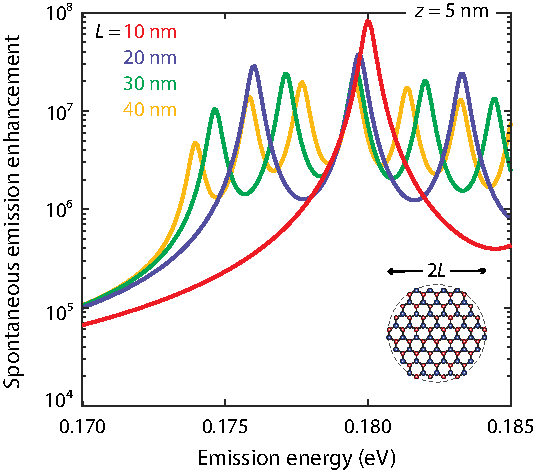
\includegraphics[width=80mm]{fig3.pdf}
    \caption{%
        \textbf{Extreme spontaneous emission enhancement due to 2D LO phonons in nanostructured geometries.} Plotted is the enhancement of the spontaneous emission rate for an emitter. The emitter is concentric with the disk and is at a distance $z=\SI{5}{\nm}$ away from the disk. For a disk with a diameter of \SI{20}{\nm}, and assuming a relaxation rate $\tau^{-1} = 5$ cm$^{-1}$, the rate of emission enhancement can be enhanced \num{100} million-fold. For an emitter with a free-space decay rate of $\SI{1e6}{\per\cm}$ at \SI{7}{\micro\m}, the emitter would experience a decay rate comparable to the frequency of the disk mode, leading to ultra-strong coupling of an external emitter with 2D LO phonons. Note that $\tau^{-1} = 5$ cm$^{-1}$ is of the order of the loss rate in bulk hBN.
        \label{fig:3}
        }
\end{figure}

\section{Strong light-matter interactions enabled by 2D optical phonons}

The extreme confinement of electromagnetic fields offered by the 2D LO phonon presents an opportunity for quantum optical applications in which one seeks to couple an external emitter such as an atom, molecule, defect, or artificial atomic system to electromagnetic fields. Applications of these couplings are ultra-bright single- or two-photon sources, realizing the strong-coupling regime and the associated phenomenology of Rabi oscillations and polaritons, or resolving spectroscopically `forbidden'' transitions \cite{koppens2011graphene,autore2018boron,rivera2016shrinking,rivera2017making,kurman2018control}.

In Figure~\ref{fig:3}, we consider the coupling of a dipole emitter to localized phonon-polaritons of nanostructured monolayer hBN. For simplicity, we consider hBN nanostructured as a disk, which leads to the formation of sharp resonances quantized along the azimuthal and radial directions. The disk is taken to have a radius of \SI{20}{cm} and a loss rate $\tau^{-1} = 5$ cm$^{-1}$, which is of the order of the loss rate in bulk hBN. In Figure~\ref{fig:3}, we plot the enhancement of the spontaneous emission rate for an external emitter polarized perpendicularly to the plane of the disk and placed \SI{5}{\nm} away from the surface of the disk. We find that the rate of spontaneous emission of 2D optical phonons is approximately 8 orders of magnitude larger than the rate of spontaneous emission of photons in the far field. For an infrared emitter at a transition wavelength of \SI{7}{\micro\m} with a free-space radiative lifetime of \SI{1}{\micro\s}, \SI{5}{\nm} away from an hBN disk, the coupling rate to 2D optical phonons (about $\SI{1e14}{\per\s}$ or 0.065 eV) would be on the same scale as the optical phonon frequency itself (about $1430$ cm$^{-1}$ or $\SI{2.70e14}{\per\s}$ or 0.18 eV). This coupling rate thus implies coupling between an emitter and the field in the regime of ultra-strong coupling. Moreover, the coupling rate for the 20 nm disk (orange), for an emitter with a far field decay rate of $> \SI{3e14}{\per\s}$ would have a sufficient coupling strength to the resonances in orange for its linewidth to span multiple resonances and thus be in a multi-mode ultra-strong coupling regime. Thus, the extreme confinement of electromagnetic energy associated with LO phonons in two dimensions enables the possibility of realizing ultrastrong coupling of an atom or molecule with optical phonons in a polar material, allowing the potential realization of new coupled states of quantum emitters and phonons such as atom-phonon polariton bound states.

The ability to probe low-loss and highly confined electromagnetic modes associated with 2D LO phonons in polar materials provides a new platform for nanophotonics in the mid- and far-infrared spectral range. The identification of the phonon-polariton of bulk and thin-film geometries with the 2D LO phonon made in this Letter would extend the rich phenomenology of optical phonons to nanophotonic applications. This work also points the way to useful new approaches to study LO phonons, arising from the fact that 2D LO phonons, unlike their 3D counterparts, have their electromagnetic energy extend a considerable distance from the material boundary. Due to the strong electromagnetic interactions between emitters and 2D LO phonons shown in this Letter, it is now possible to design interesting new hybrid states of matter and phonons based on quantum electrodynamical strong coupling. The highly confined optical phonon waves in polar monolayers may also provide interesting new opportunities in near-field radiative heat transfer, in which it has been long known that thin-film surface phonon-polaritons play a critical role. An important avenue of future study would be the \textit{ab initio} calculation of lifetimes of 2D LO phonons associated with three-phonon processes and electron-phonon interactions. In further work, it would be of great interest to study the effects of isotopic purification and cryogenic temperatures on reducing the decay rate of these 2D LO phonons.

\section{Acknowledgments}
N. R. recognizes the support of the DOE Computational Science Graduate Fellowship (CSGF) fellowship no. DE-FG02-97ER25308. T. C. acknowledges support from the Danish Council for Independent Research (Grant No.\ DFF--6108-00667). The authors thank Prof. Ido Kaminer (Technion), Siyuan Dai (Columbia), Samuel Moore (Columbia), Jennifer Coulter (Harvard), and Christopher Ciccarino (Harvard) for helpful discussions. This work was supported by the DOE Photonics at Thermodynamic Limits Energy Frontier Research Center under grant number DE-SC0019140.



\bibliographystyle{apsrev4-1}
\bibliography{references}

\end{document}
